\subsection{مقدمه}
\subsubsection{نصب Cockroach}
برای استفاده از CockroachDB 
مانند قسمت‌های قبلی، از داکر و داکرکامپوز
استفاده می‌کنیم به این صورت که ابتدا از اسکریپت
create\_cockroach\_nodes
برای ساخت تعداد دلخواه node 
استفاده می‌کنیم که این اسکریپت آنها را در یک شبکه قرار می‌دهد و نیز آنها را به یکدیگر متصل می‌کند.
\\
حال یک نمونه از فایل داکر ساخته شده برای 3 عدد node را می‌توان مشاهده کرد :
\begin{latin}
  \begin{verbatim}
    version: '3'
    services:
      roach1:
        image: cockroachdb/cockroach
        command: start --advertise-addr=roach1:26357 
                  --http-addr=roach1:8080 --listen-addr=roach1:26357 
                  --store=tpcc-local1 --sql-addr=roach1:26257 
                  --insecure --join=roach1:26357,roach2:26357,roach3:26357
        hostname: roach1
        ports:
          - "26257:26257"
          - "8080:8080"
        volumes:
          - ./cockroach-data/roach1:/cockroach/cockroach-data
        networks:
          - crdb_network
      roach2:
        image: cockroachdb/cockroach
        command: start --advertise-addr=roach2:26357
                    --http-addr=roach2:8081 --listen-addr=roach2:26357
                    --store=tpcc-local2 --sql-addr=roach2:26258
                    --insecure --join=roach1:26357,roach2:26357,roach3:26357
        hostname: roach2
        ports:
          - "26258:26258"
          - "8081:8081"
        volumes:
          - ./cockroach-data/roach2:/cockroach/cockroach-data
        networks:
          - crdb_network
      roach3:
        image: cockroachdb/cockroach
        command: start --advertise-addr=roach3:26357
                    --http-addr=roach3:8082 --listen-addr=roach3:26357
                    --store=tpcc-local2 --sql-addr=roach3:26259
                    --insecure --join=roach1:26357,roach2:26357,roach3:26357
        hostname: roach3
        ports:
          - "26259:26259"
          - "8082:8082"
        volumes:
          - ./cockroach-data/roach3:/cockroach/cockroach-data
        networks:
          - crdb_network
    networks:
      crdb_network:
        driver: bridge

  \end{verbatim}
\end{latin}

\noindent
یکی از دلایلی که cockroach 
دیتابیس توزیع شده خوبی است این است که برخلاف cassandra 
که هر node آن مقدار
زیادی منبع مصرف می‌کند، این دیتابیس بسیار در مصرف منابع بهینه عمل می‌کند به صورتی که تقریبا روی کانفیگ من که در ابتدای گزارش گفته شد، حدود ۱۲ node با عملکرد بسیار خوب می‌توان داشت.
\\
حال پس از راه‌اندازی node ها اسکریپت benchmark.sh را ران می‌کنیم که 
تست TPC-C 
را اجرا می‌کند.
این تست یکی از معتبرترین و واقعی‌ترین تست‌های دیتابیس‌های توریع‌شده است که 
یک فروشگاه آنلاین را به همراه تعداد انبار داده شده مثلا آمازون و تراکنش‌های آن، شبیه‌سازی می‌کند.
برای اطلاع بیشتر از این تست بسیار جالب به 
\link{https://www.tpc.org/tpc_documents_current_versions/pdf/tpc-c_v5.11.0.pdf}{این لینک}
مراجعه کنید.
\\
طبق عکس زیر مشاهده می‌کنیم که برای تست به صورت لوکال باید از ۳ 
node استفاده کنیم.
\\
\begin{figure}[H]
  \centering
  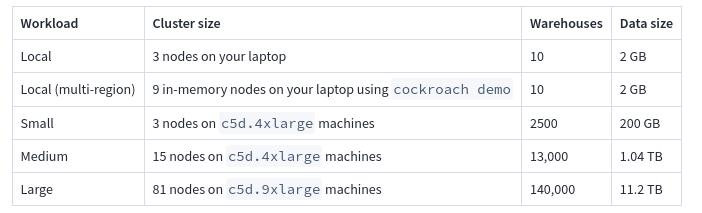
\includegraphics[scale=0.5]{pictures/cockroach/init/tpcc2.png}
  \caption{تنظیمات \lr{benchmark}}
\end{figure}
حال برای انجام این تست ابتدا باید در یکی از node 
های کلاستر، داده‌های تست را لود کنیم و دیتابیس را بسازیم.
\\
\codebox{
  cockroach workload fixtures import tpcc --warehouses=10 'postgresql://localhost:26257?sslmode=disable'
}
\begin{figure}[H]
  \centering
  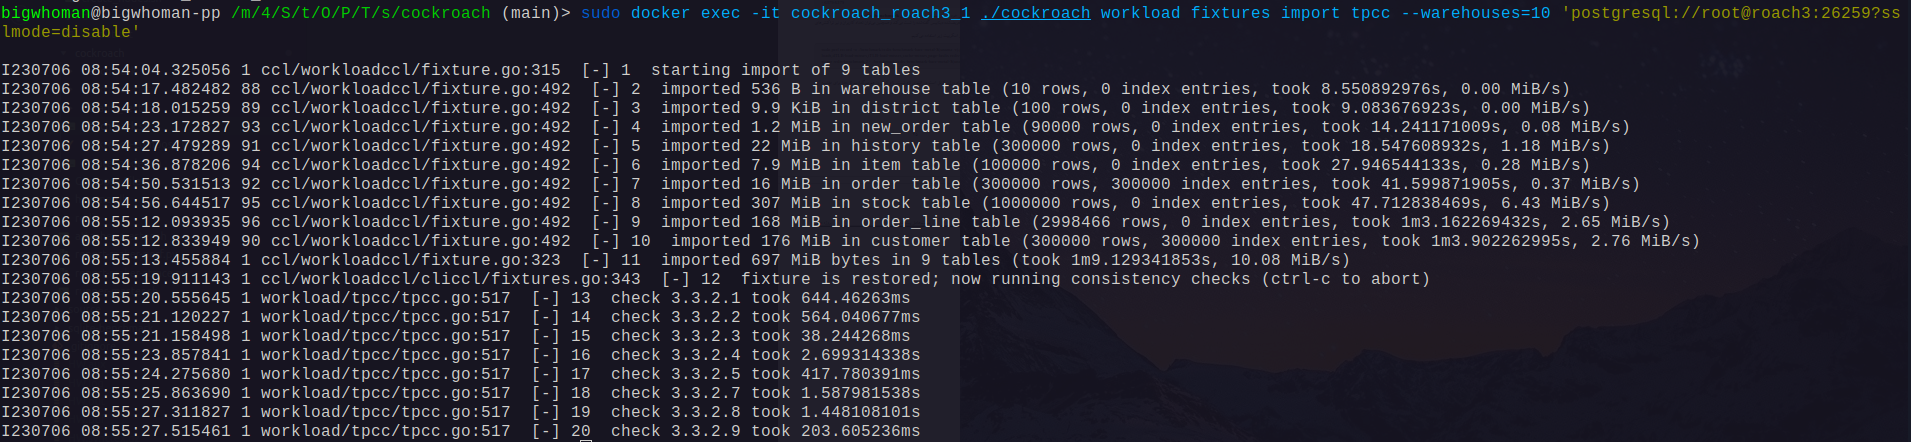
\includegraphics[scale=0.25]{pictures/cockroach/init/init-tpcc2.png}
  \caption{نتیجه import داده}
\end{figure}
سپس تست را با دستور زیر شروع می‌کنیم.
این تست به مدت ۱۰ دقیقه اجرا می‌شود.
\codebox{
cockroach workload run tpcc --warehouses=10 --ramp=3m --duration=10m 'postgresql://localhost:26257?sslmode=disable' >./output.txt
}
در ادامه از کدهای زیر برای attach کردن perf, strace به پردازه‌ها استفاده می‌کنیم.
\codebox{
  sudo perf record -p \$(pidof cockroach | cut -d' ' -f2- | tr ' ' ',') -o ./benchmark/cockroach-benchmark-tpcc-bare-metal-\$(uname -r).perf -e tlb:tlb\_flush,dTLB-loads,dTLB-load-misses,iTLB-load-misses,cache-misses,page-faults
}
\codebox{
 strace -f -p "\$(pidof cockroach | cut -d' ' -f2- | tr ' ' ',')" 2> ./benchmark/cockroach-benchmark-tpcc-bare-metal-\$(uname -r).strace
}

نتایج کلی مانند دو دیتابیس قبلی یعنی ردیس و کاساندرا است و دلیل هم مانند دو سیستم قبلی عدم وجود منابع کافی برای ماشین مجازی است.